%\vspace{-1ex}
\section*{\sout{Appendix: Additional Line Simplification Algorithms}}
Apart from the techniques evaluated in this article, there exist other approaches for various requirements of trajectory compression.
We next summarized some of the representative \lsa algorithms. Interested readers may refer to \cite{Shi:Survey, Muckell:Compression, Lin:Cised, Zhang:Evaluation} for more details. %related work.




%\subsection*{A.1 Other Line simplification algorithms}

\stitle {\sout{Weak simplification algorithms.}}
Weak simplification allows that the output data points may not belong to the original data sets \cite{Trajcevski:DDR} (otherwise, the strong simplification).
That is, weak simplification allows data interpolation. Algorithms \sleeve \cite{Zhao:Sleeve}, \operb\cite{Lin:Operb} and \cised \cite{Lin:Cised} are both strong and weak \lsa algorithms whose weak versions have better compression ratios than their strong counterparts, and even comparable with the optimal algorithms \cite{Lin:Cised}.

\stitle {\sout{Algorithms using other error metrics.}} %on the min-$\#$ problem
A number of algorithms \cite{Agarwal:Metric, Chen:Fast, Wu:Graph,Cao:Dots} have been developed to solve the ``min-\#" problem under alternative error metrics.
\cite{Agarwal:Metric} studies the problem under the $L_1$ and uniform (also known as Chebyshev) metric. % while this study focuses on the $L_2$ metric.
\cite{Chen:Fast} defines \eat{the local integral square synchronous Euclidean distance (LISSED) and} the integral square synchronous Euclidean distance (\kw{ISSED}), an accumulation of square \sed, and uses it to speed up the construction of reachability graphs, \cite{Wu:Graph} follows the ideas of \cite{Chen:Fast} and Dots \cite{Cao:Dots} is an online \eat{and near-optimal} trajectory simplification algorithm that uses \kw{ISSED}.
Note that these error metrics are not as popular as \ped and \sed.
%Note these error metrics have varied effectiveness compared with \ped and \sed.


\stitle {\sout{Algorithms on the min-$\epsilon$ problem.}}
Some studies focus on the min-$\epsilon$ problem \cite{Chan:Optimal} that, given $m$, constructs an approximate curve consisting of at most $m$ line segments with the minimum error. SQUISH($\lambda$) \cite{Muckell:SQUISH} and SQUISH-E($\lambda$) \cite{Muckell:Compression} are such algorithms that compress a trajectory of length $n$ into a trajectory of length at most $n/\lambda$.
These methods lack the capability of compressing trajectories while ensuring that \sed errors are within a user-specified bound \cite{Muckell:Compression}.
%It is based on the priority queue data structure, where the prioritization is determined based on estimating the amount of \sed introduced into the compression if that point was removed from the compression\cite{Muckell:SQUISH}.




\eat{
\subsection*{A.2 Semantic based algorithms}
The trajectories of certain moving objects such as cars and trucks are constrained by road networks. These moving objects typically travel along road networks, instead of the line segment between two points. Trajectory compression methods based on road networks \cite{Chen:Trajectory, Popa:Spatio,Civilis:Techniques,Hung:Clustering, Gotsman:Compaction, Song:PRESS, Han:Compress}  project trajectory points onto roads (also known as Map-Matching). Moreover, \cite{Gotsman:Compaction, Song:PRESS, Han:Compress} mine and use high frequency patterns of compressed trajectories, instead of roads, to further improve compression effectiveness.
%
Some methods \cite{Schmid:Semantic, Richter:Semantic} compress trajectories beyond the use of road networks, and further make use
of other user specified domain knowledge, such as places of interests along the trajectories \cite{Richter:Semantic}.
%
There are also compression algorithms preserving the direction of the trajectory \cite{Long:Direction}. %As it mentions that the trajectory of a moving object contains a large amount of semantic information that could be used to compress the trajectory. For example, the driving direction of a moving object implies the information of the next direction.

These  semantics based approaches are orthogonal to line simplification based methods, and may be combined with each other to  improve the effectiveness of trajectory compression.
}





%%%%%%%%%%%%%%%%%%%%%%%%%%%%%%%%%%%%%%%%End%%%%%%%%%%%%%%%%%%%%%%%%%%%%%%%%%%%%%%%%%%%%%%%%%%%%%%%%%%
\eat{
\textcolor[rgb]{1.00,0.00,0.00}{The one-pass line simplification algorithms are originally developed in disciplines of computational geometry and cartography. As summarized in \cite{Shi:Survey}, they are five categories of one pass line simplification algorithms, namely independent point algorithms, uniform sampling, local processing routines, strip routines and sleeve routines.
	Note that in \cite{Shi:Survey}, the strip and sleeve routines are classified into the same category, called unconstrained extended local processing.
	These routines all use the \ped metric if an error metric is needed.}
}






\eat{%%%%%%%%%%%opening window
	\stitle{Opening Window}.
	The \opwa algorithm~\cite{Meratnia:Spatiotemporal} combines the Top-down and opening window strategies, and enforces the constrained global checking in the window.
	
	Given a trajectory $\dddot{\mathcal{T}}[P_0, \ldots, P_n]$ and an error bound $\zeta$, algorithm \opwa~\cite{Meratnia:Spatiotemporal} maintains a window $W[P_s, \ldots, P_k]$, where $P_s$ and $P_k$ are the start and end points, respectively. Initially, $P_s$ = $P_0$ and $P_k$ = $P_1$, and the window $W$ is gradually expanded by adding new points one by one. \opwa tries to compress all points in $W[P_s, \ldots, P_k]$ to a single line segment $\mathcal{L}(P_{s}, P_{k})$. If the distances $ped(P_i, {\mathcal{L}})\le \zeta$ for all points $P_i$ ($i\in[s, k]$), it simply expands $W$ to $[P_s, \ldots, P_k, P_{k+1}]$ $(k+1\le n)$ by adding a new point $P_{k+1}$. Otherwise, it produces a new line segment $\mathcal{L}(P_{s}, P_{k-1})$, and replaces $W$ with a new window $[P_{k-1},\ldots,P_{k+1}]$. The above process repeats until all points in $\dddot{\mathcal{T}}$ have been considered.
	
	%\textcolor[rgb]{0.00,0.07,1.00}{According to the different methods of selecting the end points of a line segment, Open Window can further be divided into Normal Penning Window and Before Opening Window~\cite{Meratnia:Spatiotemporal}. When the distance of the point to compressed trajectory exceeds a certain threshold, Normal Opening Window algorithm select that point as the end point, while Before Opening Window select the last point within the window as the end point of the current trajectory.}
	
	Algorithm \opwa is not efficient enough for compressing long trajectories as it remains in $O(n^2)$ time, the same as the \dpa algorithm.
	Also, \ped and \sed are both supported in \opwa as the algorithm \dpa does.
}%%%%%%%%%%%opening window

\eat{%%%%%%%%%%%sliding window
	\stitle{Sliding Window}.
	The Lang simplification algorithm\cite{Lang:SideWindow}, is similar to the opening window approach except that a window is initialized as a region containing a fixed number of consecutive original points.
	%If the distance from the segment, which connects the first and last original points inside the window, to the individual original points between the segment��s endpoints is less than the tolerance, a new window will be initialized by setting the last original point as the starting point; Otherwise, the window will be updated by excluding the last original point. The window is shifted over the original line.
	
	The \swab algorithm~\cite{Keogh:online} is essentially the combination of the Sliding Window mechanism and the Bottom-up algorithm.
	It keeps a window, $w[P_s, \ldots, P_{s+k-1}]$, of a fixed size of $k$.
	The window size $k$ should be carefully chosen so that there are enough data points in the window to create about 5 or 6 line segments \cite{Keogh:online}.
	Initially, $P_s=P_0$.
	Next, the Bottom-Up algorithm, \eg \pavlidis algorithm, is applied to the points in the window, which merges the points into segments with the left-most segment being $\vv{P_sP_{s+i}}$, $i<k$.
	Then $\vv{P_sP_{s+i}}$ is output, the window slides to right taking $P_{s+i+1}$ as the new start point of the window, and the Bottom-Up algorithm is applied again.
	This process repeated until all points have been merged to segments.
	
	The time complexity of \swab is a small constant factor worse than that of the standard Bottom-Up algorithm~\cite{Keogh:online}.
	Also, it supports \sed. % as the standard Bottom-Up algorithm does.
	
	\textcolor[rgb]{1.00,0.00,0.00}{Todo...dis-continuous line segments.}
	
}%%%%%%%%%%%sliding window


\eat{ %%%%%%%%%%%%%%%%%%%%%%%%%strip and LDR
	
	\stitle{Reumann-Witkam}.
	In Reumann-Witkam\cite{Reumann:Strip}, the input data is divided into sections by \emph{strips}.
	Initially, the first \emph{strip}, with the width of $2*\epsilon$, takes the line $\vv{P_0P_1}$ connecting the first two points, $P_0$ and $P_1$ as its middle line.
	Then the \emph{strip} is expending over the line into the direction of its initial tangent, covering the succeed points, $P_2, \ldots, P_{j}$, until the \emph{strip} hits the line $\vv{P_jP_{j+1}}$ (meaning that the next point $P_{j+1}$, $j>1$, is out side of the \emph{strip}).
	The points, $[P_0, \ldots, P_{j}]$, within this \emph{strip} compose a section. The first and last points of the section, \ie $P_0,P_{j}$, are output, and those points between them are removed.
	The last point $P_{j}$ is the initial point of the next \emph{strip}.
	The whole process is repeated until the strip contains the end point $P_n$ of the input data.
	The Reumann-Witkam algorithm is a one-pass algorithm.
	
	\textcolor[rgb]{1.00,0.00,0.00}{The Opheim simplification algorithm \cite{Opheim:Reduction} defines the search region (\ie slide window) in a similar manner as the strip of Reumann-Witkam.}
	
	
	\stitle{Line Dead Reckoning}.
	Line Dead Reckoning (LDR)\cite{Lange:Tracking} is a policy which essentially represents an agreement between a given moving object and the Moving Object Database (MOD) server.
	The agreement specifies a threshold $\zeta$ that is a parameter of the policy.
	%Each moving object is aware about its actual location by periodically sampling it.
	Initially, the moving object sends a tuple $(x_0, y_0, t_0, \vv{v}_0)$ to the MOD, denoting the initial expected velocity $\vv{v}_0$ of the object at certain location $(x_0, y_0)$ and time $t_0$. The server estimates the future track of that object by straightly extrapolating from the tuple currently received.
	For the object, if its actual location at a given time $t_i$ does not deviate by more than $\zeta$ from the location $(x_i, y_i)$ at $t_i$ estimated by the same policy using the tuple previously transmitted, the object does not transmit any new updates to the MOD server. Otherwise, the object will send another tuple $(x_i, y_i, t_i, \vv{v_i})$ to the MOD server. Note that the deviation metric here is equivalent to the \sed.
	
	
	In \cite{Trajcevski:DDR}, the authors proved that the LDR method is not only a policy to track the current position of a moving object, but also an error bounded way (\sed error bounded by the parameter $\zeta$) to online compress the trajectory of the object, as long as the algorithm uses $\zeta/2$ as the tolerance threshold. Indeed, it is the first \sed error-bounded and one-pass trajectory simplification algorithm for trajectory compression. However, its compression ratios are obvious poor, because the tolerance threshold is the half of the $\zeta$ and both the value and the direction of the velocity are pre-defined and fixed between two updates.
} %%%%%%%%%%%%%%%%%%	
	
	
\eat{ %%%%%%%%%%%%%%%%%%%%%%%%%Examples of strip and LDR	
	\begin{figure*}[tb!]
		\centering
		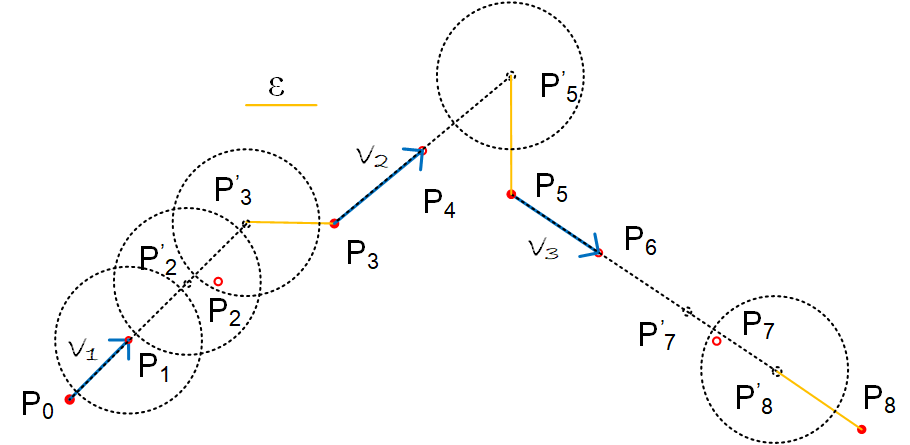
\includegraphics[scale=0.66]{figures/Fig-LDR.png}
		\vspace{-1ex}
		\caption{\small The trajectory $\dddot{\mathcal{T}}[P_0, \ldots, P_{10}]$ is compressed by the Reumann-Witkam and Linear Dead Reckoning algorithms to four and eight line segments, respectively.}
		\vspace{-2ex}
		\label{fig:ldr}
	\end{figure*}
	
	\begin{example}
		\label{exm-alg-strip}
		In Figure~\ref{fig:ldr}, the trajectory $\dddot{\mathcal{T}}[P_0, \ldots, P_{10}]$ is compressed
		%
		(1) by the Reumann-Witkam to four line segments $\vv{P_0P_2}$, $\vv{P_2P_4}$, $\vv{P_4P_7}$ and $\vv{P_7P_{10}}$. First, a strip with width $2\epsilon$ is built parallel to the line $\vv{P_0P_1}$, then the strip is extended over the line and includes point $P_2$. Because $P_3$ is outside of the strip, $P_2$ becomes the end point of the first section and the start point of the second section.
		%
		(2) by the Linear Dead Reckoning algorithm to eight line segments $\vv{P_0P_1}$, $\vv{P_1P_2}$, $\vv{P_2P_3}$, $\vv{P_3P_4}$, $\vv{P_4P_5}$, $\vv{P_5P_7}$, $\vv{P_7P_8}$ and $\vv{P_8P_{10}}$. First, an initial velocity ${\vv{v}_0}$ is set to $|P_0P_1|/(t_1-t_0)$. Then the synchronized point $P'_2$ of $P_2$ is estimated based on the velocity ${\vv{v}_0}$ and time of $P_2$, \ie ${v}_0 * (t_2-t_0)$. Because the \sed from $P_2$ to the line $\vv{P_0P'_2}$ , \ie $|P_2P'_2|$, is great than $\epsilon/2$, the algorithm outputs $\vv{P_0P_1}$ and starts the next section.
	\end{example}
}%%%%%%%%%%%%%%%%%%%%%%%%%Examples of strip and LDR



\eat{%%%%%%%%%%%%%%%%%%%%%%%%%
\subsection*{A.3 Wild algorithms}

\stitle{Independent point algorithms}.
\textcolor[rgb]{0.00,0.07,1.00}{Independent point algorithms roughly determine which points of a line should be retained. Two examples of this category are the $n^{th}$ point routine and the routine of random-selection of points \cite{Shi:Survey}. In these two routines, for every fixed number of consecutive points along the line, the $n^{th}$ point and one random point among them are retained, respectively.}

\stitle{Naive Local Processing}.
\textcolor[rgb]{0.00,0.07,1.00}{The Naive local processing routines\cite{Shi:Survey} regards a relationship between every two or three consecutive original points. Two examples of the relation are (a) the distance between the two consecutive points and (b) the perpendicular distance from a line connecting two points to an intermediate point, which should not be smaller than their individual tolerance bandwidths (a user-supplied minimum distance or angular change). Points within the bandwidth are eliminated, whereas points exceeding the bandwidth are retained. These tolerance routines are called the routine of distance between points and the perpendicular distance routine, respectively.}

\stitle{Uniform Sampling}.
\textcolor[rgb]{0.00,0.00,1.00}{Similarly, Uniform Sampling\cite{Muckell:Compression} down samples a trajectory \trajec{T} at fixed time intervals in a manner that achieves the compression ratio of $\lambda$.}
}%%%%%%%%%%%%%%%%%
